Boom hacka lacka

\subsubsection{Shadows}
Shadows are one those things that can make a scene really come to life. There are many techniques in which shadows can be achieved with different pros and cons. We have chosen to use shadow mapping since it offers real-time shadows for arbitrary shapes in a theoretically straight forward way. 

The quality of these can be increased arbitrarily, but the computational complexity is increased equivalently, which is what limits this method. 

More specifically our implementation utilizes \textit{Light-Space Shadow Mapping} which can be summarized in the following steps:

\begin{itemize}
\item Place the camera in the light source and adjust the camera frustum to cover the part of the scene that will be visible in the final render.
\item Render the scene with as simple shaders as possible and store the depth buffer. This is the shadow map.
\item Place the camera in its final-render location.
\item For each vertex:
\begin{itemize}
\item Transform into light-space coordinates.
\item Compare the distance from the light source with the corresponding value in the shadow map.
\item If the vertex is further away than the shadow map suggests, it will be shadowed. 
\end{itemize}
\end{itemize}



\subsubsection{Fog}
The transition between different parts of the world can sometimes be very sharp in an unpleasant way. For instance, at the border between the sky and the ocean seen in figure \ref{fig:HorizonNoFog}. 

This can be remedied be adding some distance-fog to the ocean. If the color of the fog matches the color of the skybox at its horizon the transition will be seamless. Our skybox has been modify to fade into the color of the fog at its horizon, which can be seen in figure \ref{fig:SkyboxComparison} below. Notice that we have chosen to not let the skybox be affected by any fog. By doing so one can always see the sky when looking up, which is rather pleasant. 

\begin{figure}[H]
\begin{subfigure}{.5\textwidth}
  \centering
  \includegraphics[width=0.9\linewidth]{images/horizonNoFog.png}
  \caption{Horizon without fog}
  \label{fig:HorizonNoFog}
\end{subfigure}%
\begin{subfigure}{.5\textwidth}
  \centering
  \includegraphics[width=0.9\linewidth]{images/horizonFog.png}
  \caption{Horizon with fog}
  \label{fig:HorizonFog}
\end{subfigure}
\caption[Noise comparison]{\textit{Comparison of noise functions}}
\label{fig:HorizonFogComparison}
\end{figure}

\begin{figure}[H]
\begin{subfigure}{.5\textwidth}
  \centering
  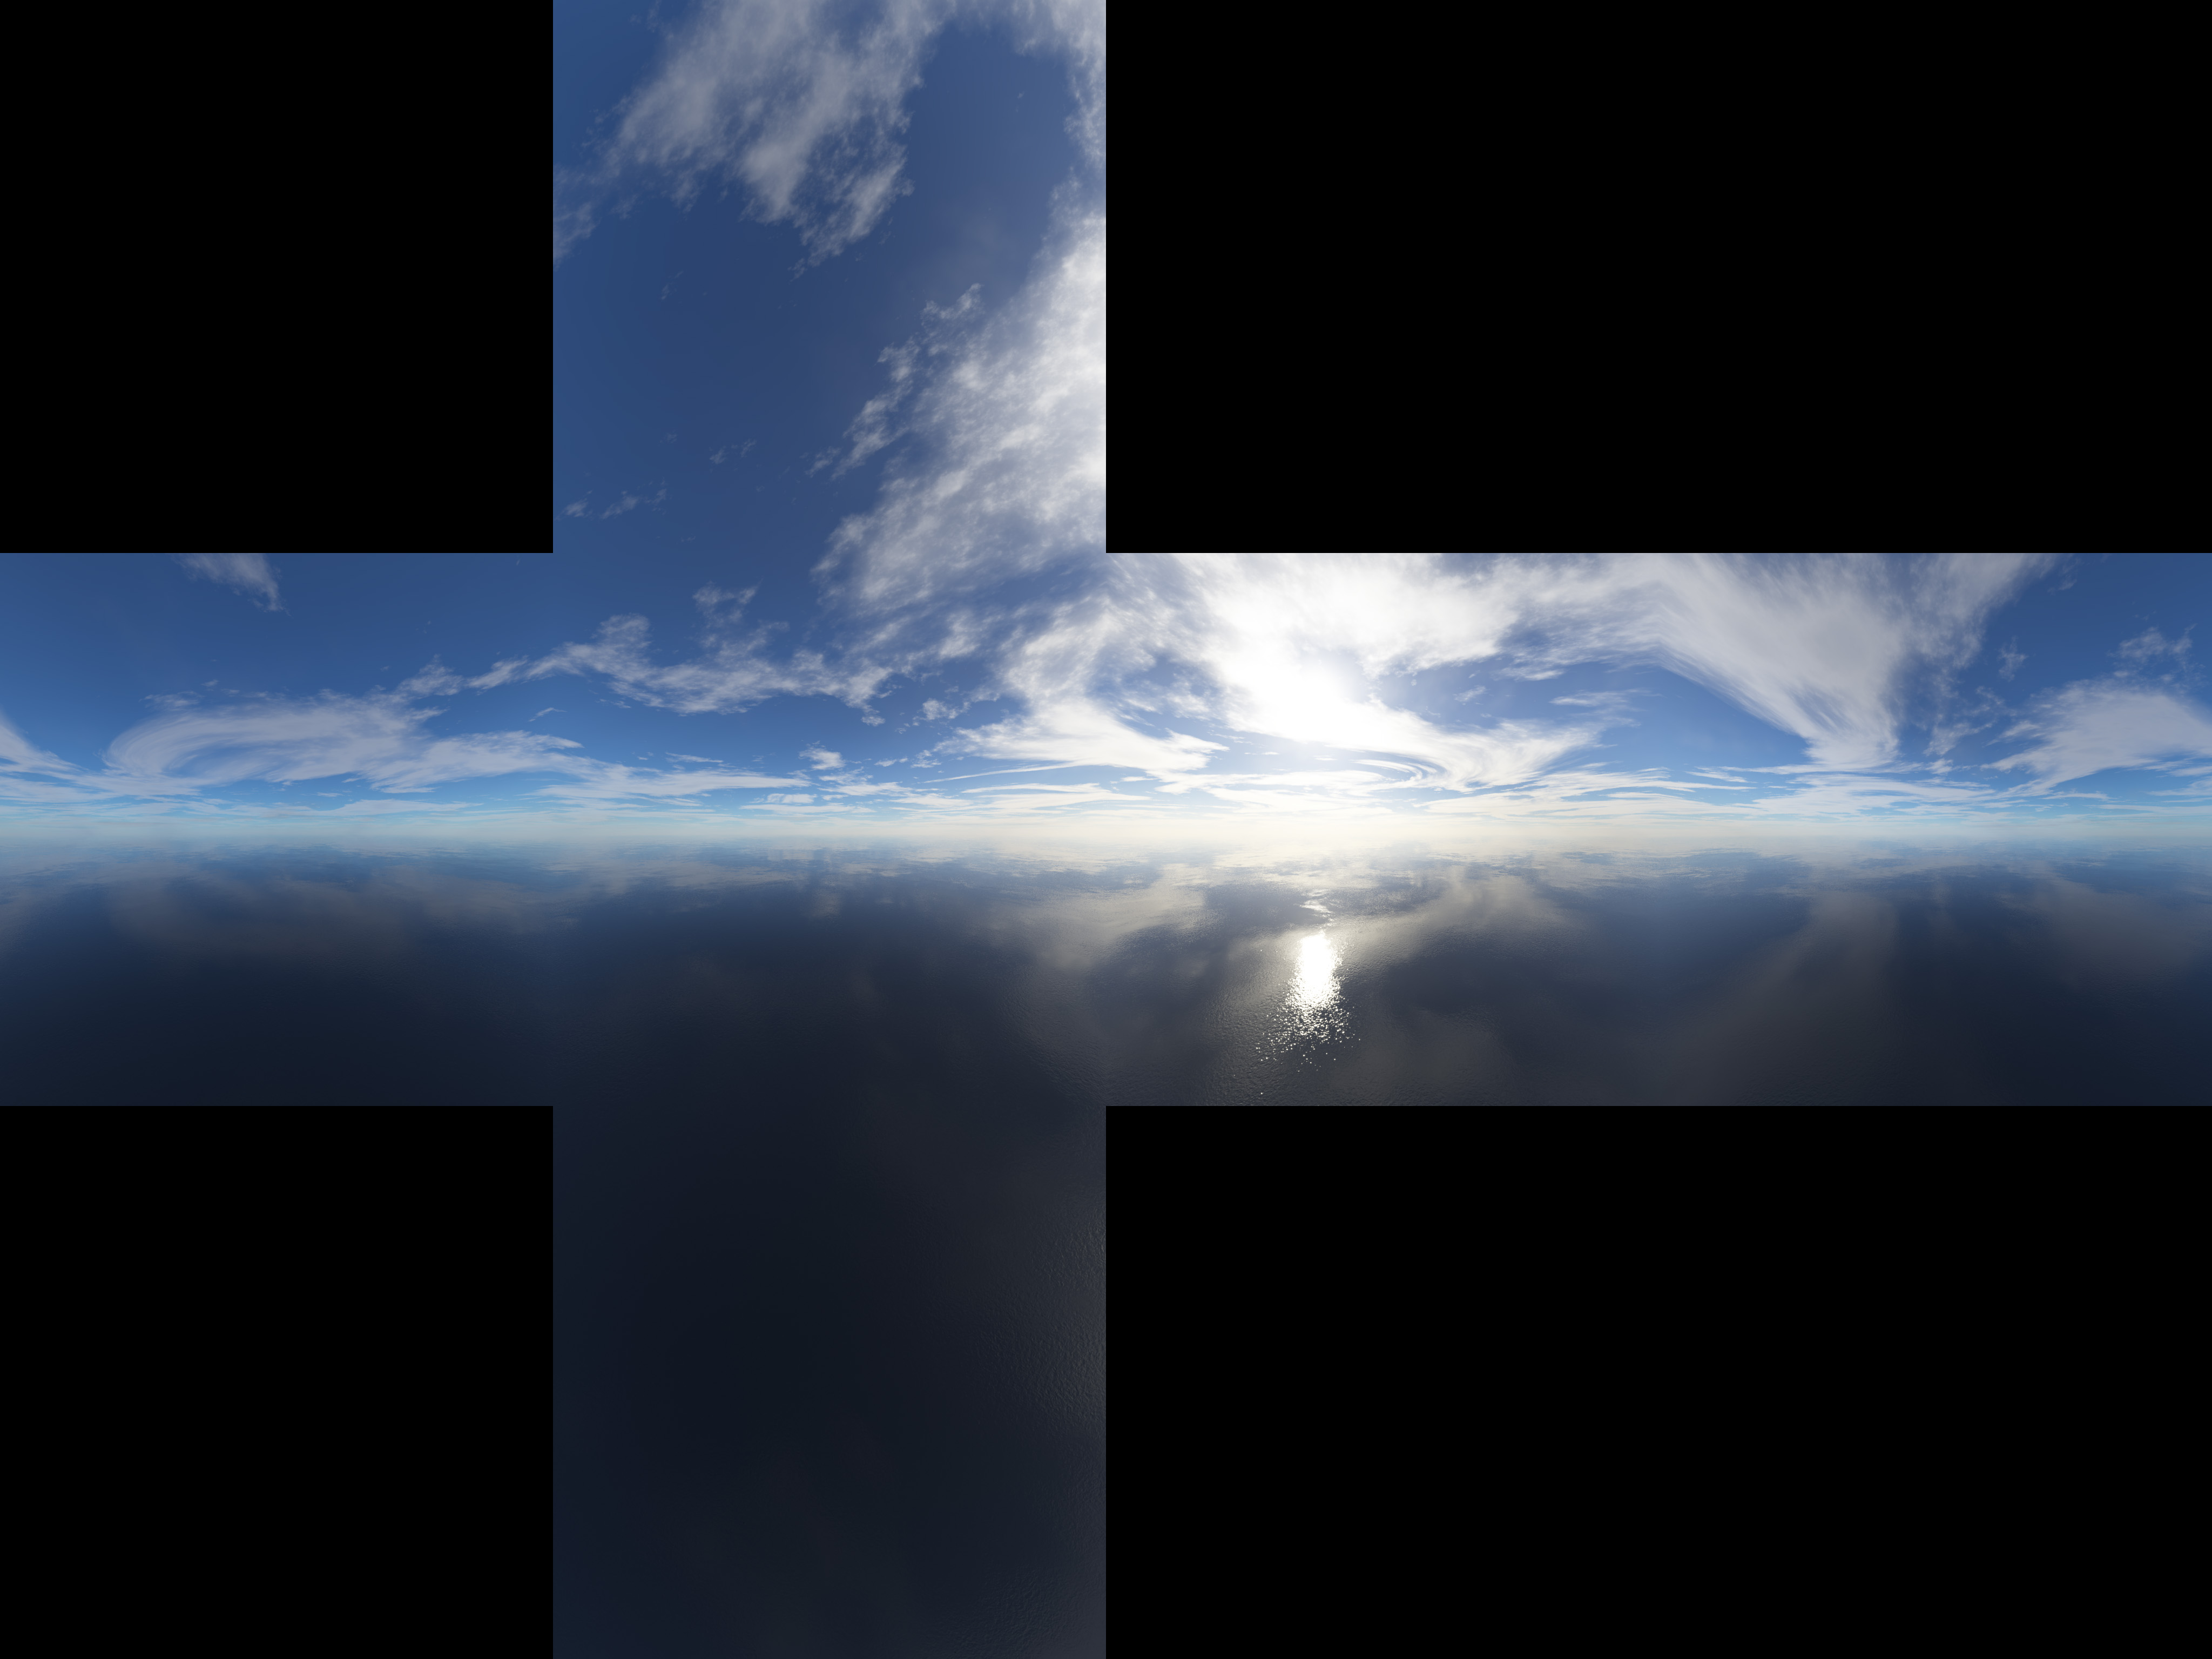
\includegraphics[width=0.9\linewidth]{images/skybox0.png}
  \caption{Original skybox}
  \label{fig:skybox0}
\end{subfigure}%
\begin{subfigure}{.5\textwidth}
  \centering
  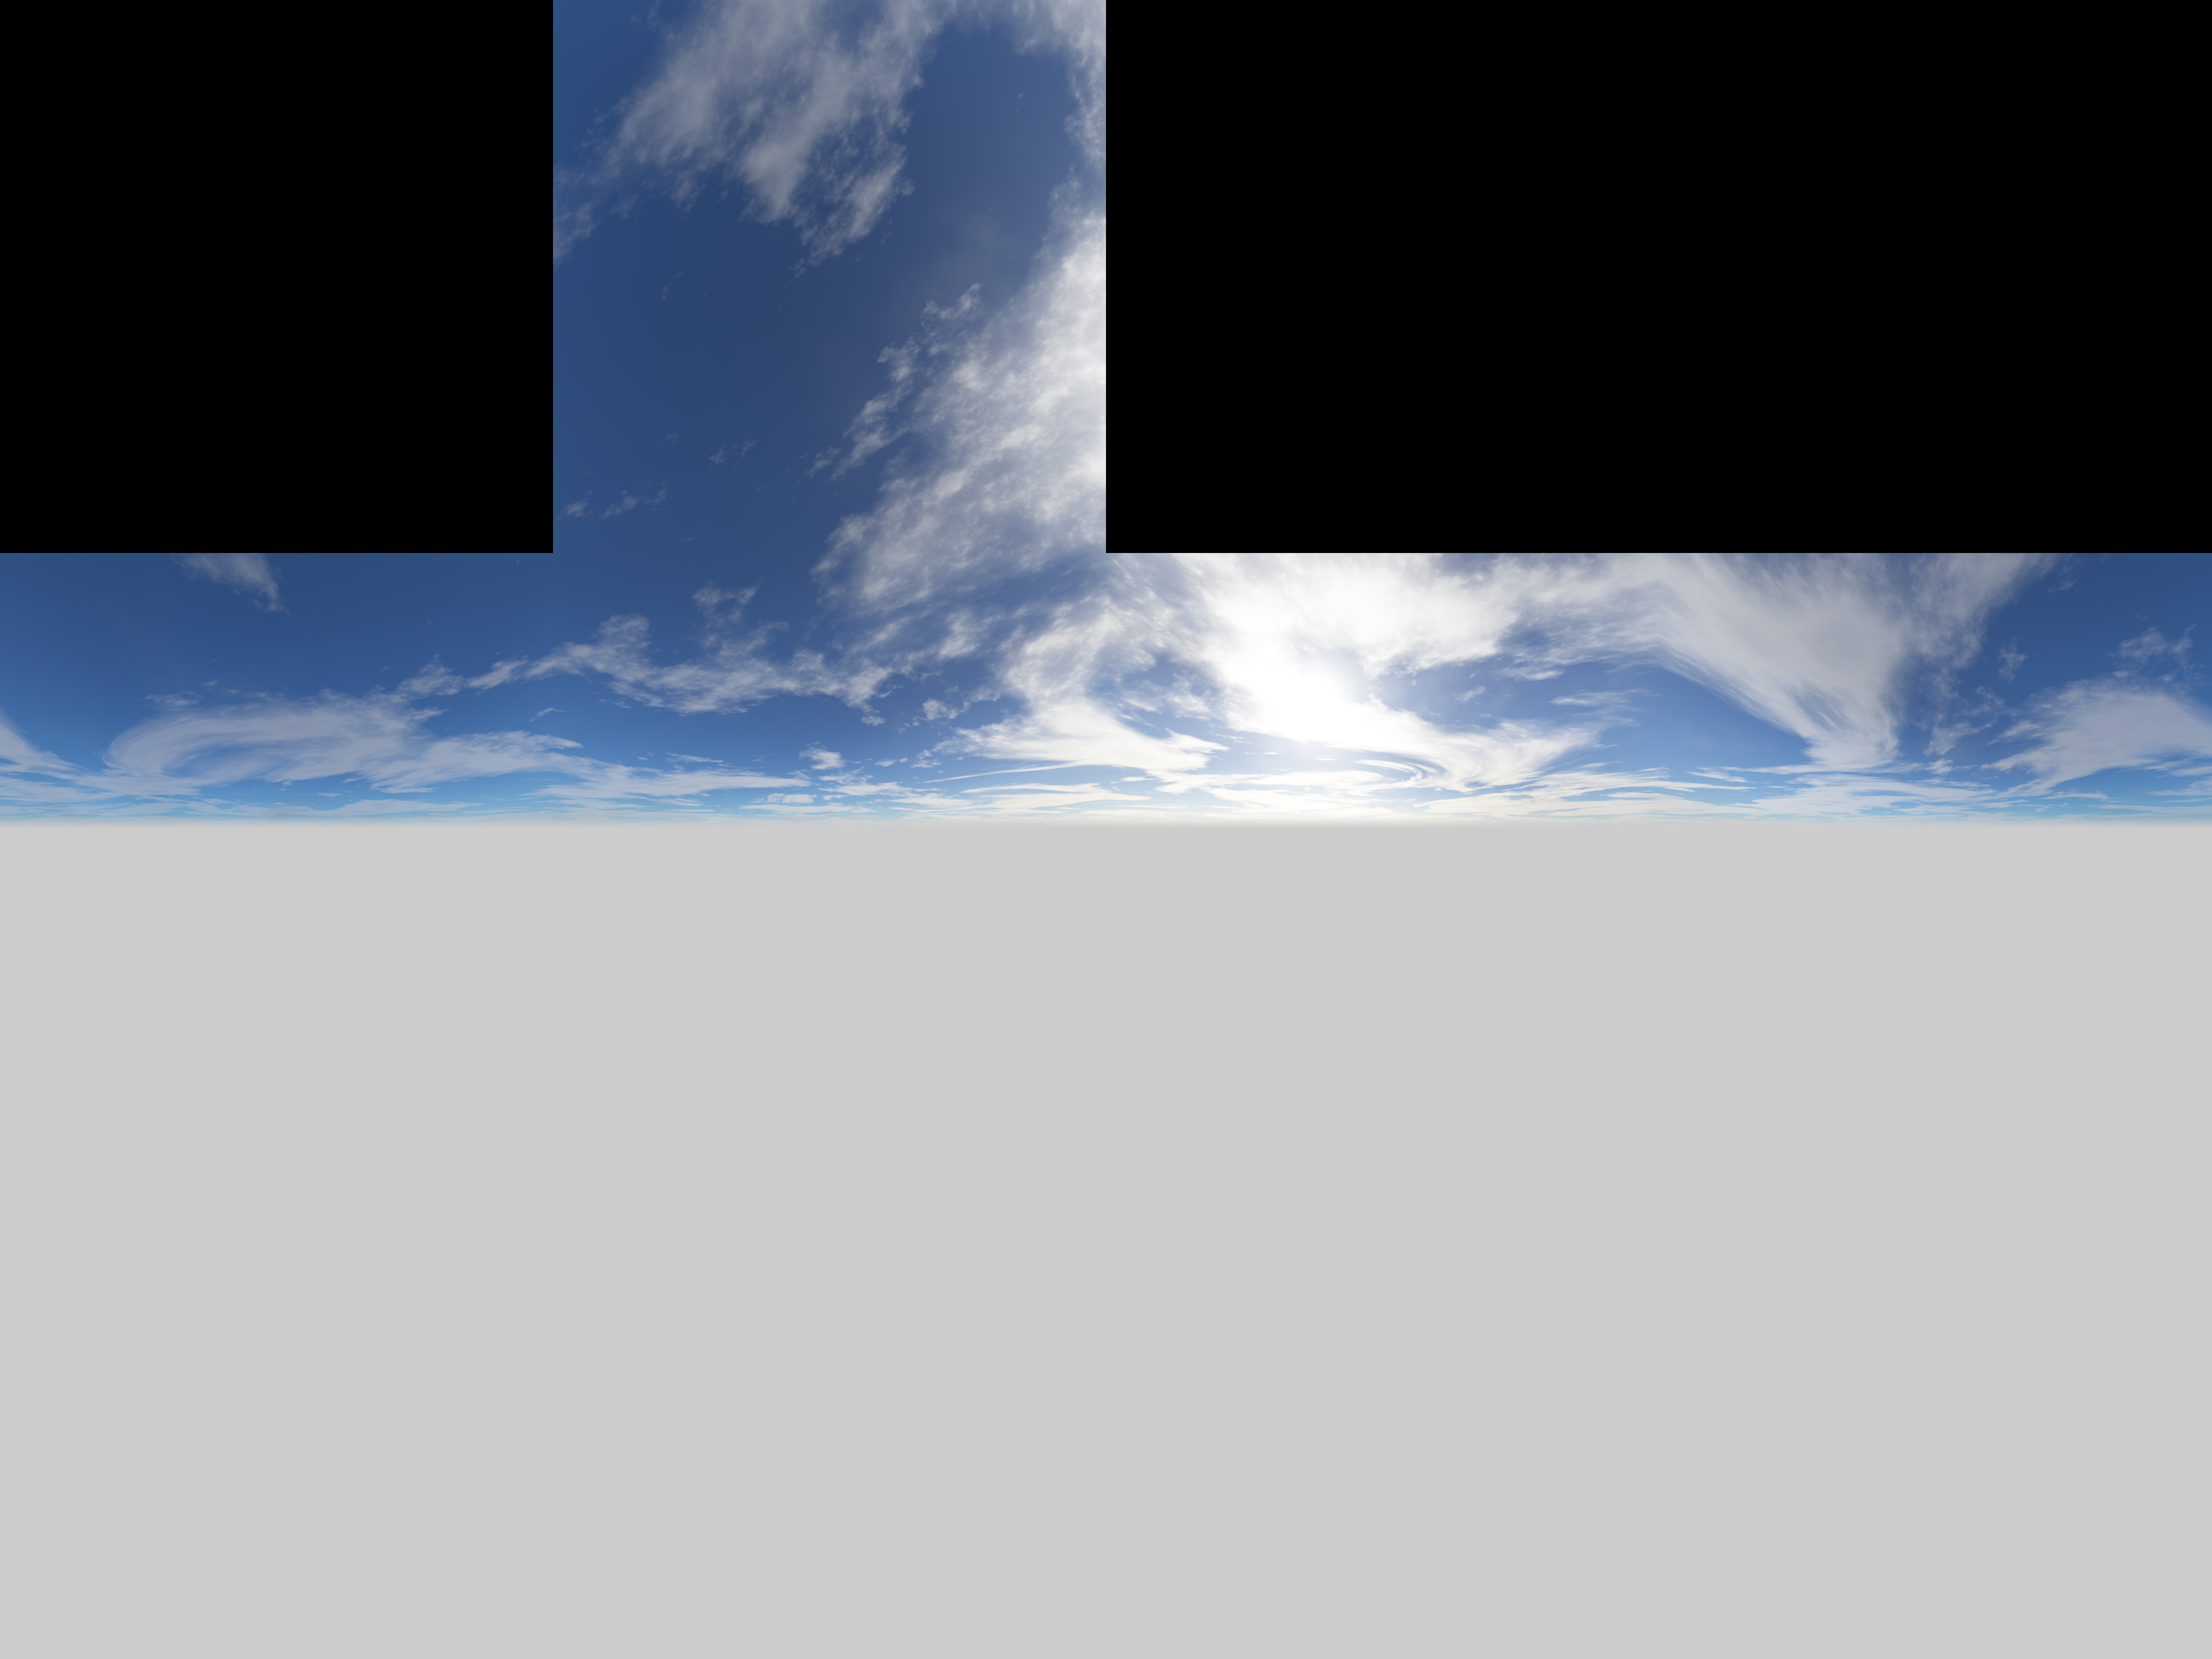
\includegraphics[width=0.9\linewidth]{images/skybox1.png}
  \caption{Skybox modified to fade into fog}
  \label{fig:skybox1}
\end{subfigure}
\caption[Noise comparison]{\textit{Comparison of skyboxes}}
\label{fig:SkyboxComparison}
\end{figure}

The distance-fog is also good for constraining the rendering size of the current scene. By adjusting the distance at which the fog appears one can adjust how much that is needed to be rendered of the scene. This enables an arbitrarily large world to be present without killing your computer since only the visible part of the world inside the fog-limit needs to be rendered. 

\subsubsection{Normal Mapping}
Normal mapping is a technique for adding fine details to an object without adding more vertices, which saves a lot of geometry computations. A normal map is generally an image where the RGB-channels represent x,y and z coordinates for a normal vector. This texture is used in the fragment shader when computing the shading for the current fragment. Before calculating the shading the normal vector is rotated to match the object on which it is to be mapped. Notice that the normal vector is not translated since we want it to remain as an normalized direction and nothing more. An example of a normal map can be seen in figure //TODO below.

// FIGURE